\chapter{Numerical results of DNS simulations} % (fold)
\label{cha:numerical_results}

\section{Backward facing step} % (fold)
\label{sec:backward_facing_step}

Numerical results of:
\begin{itemize}
\item DNS-simulations
\item an algebraic simulation
\item a \ke-simulation
\end{itemize}
were compared with experimental results given us by the department for aerodynamics. Because of its transient character, we also performed a stochastic analysis of the DNS simulations. All simulations were performed in 2D.

\subsubsection*{DNS-simulations}

For DNS, 3 simulations with different inlet velocities were performed ($u=3.372,/s$, $=5.295,/s$, $=5.579,/s$).

\noii The flow in the DNS-simulations is highly transient: vortices and secondary vortices are created periodically behind the step. They are dragged by the main flow down the channel. Also vortices appear at the top wall. To be able to make reasonable conclusions, we performed a stochastic analysis. The stochastic moments of the simulation were inserted into the same plot as the ones of the experimental results (see figure~\ref{fig:bfsA}, \ref{fig:bfsB} and \ref{fig:bfsC}). 

\noii It can be well seen that the maximum mean velocity tends to the bottom wall in the experiment after the step. This extreme behaviour could not be encountered in the simulation: the maximum velocity shifts gradually to the middle of the channel\footnote{The integral of the mean velocity over the paths seem to increase with increasing position x. Maybe the assumption of an incompressible flow is not given.}. The mean reattachment length for $u=3.372m/s$ could be determined to be between positions D and E. This is much longer as the reattachment length of the experiment.

\noii Please note that the variance at the inlet of the experimental backward facing step is quite high\footnote{No velocity fluctuation was assumed at the inlet of the simulations.}. This and different vortex patterns downstream of the step might be the reason for the discrepancy of the mean flow profile and the attachment length.

\newpage

\begin{figure}[!htb]
\centering
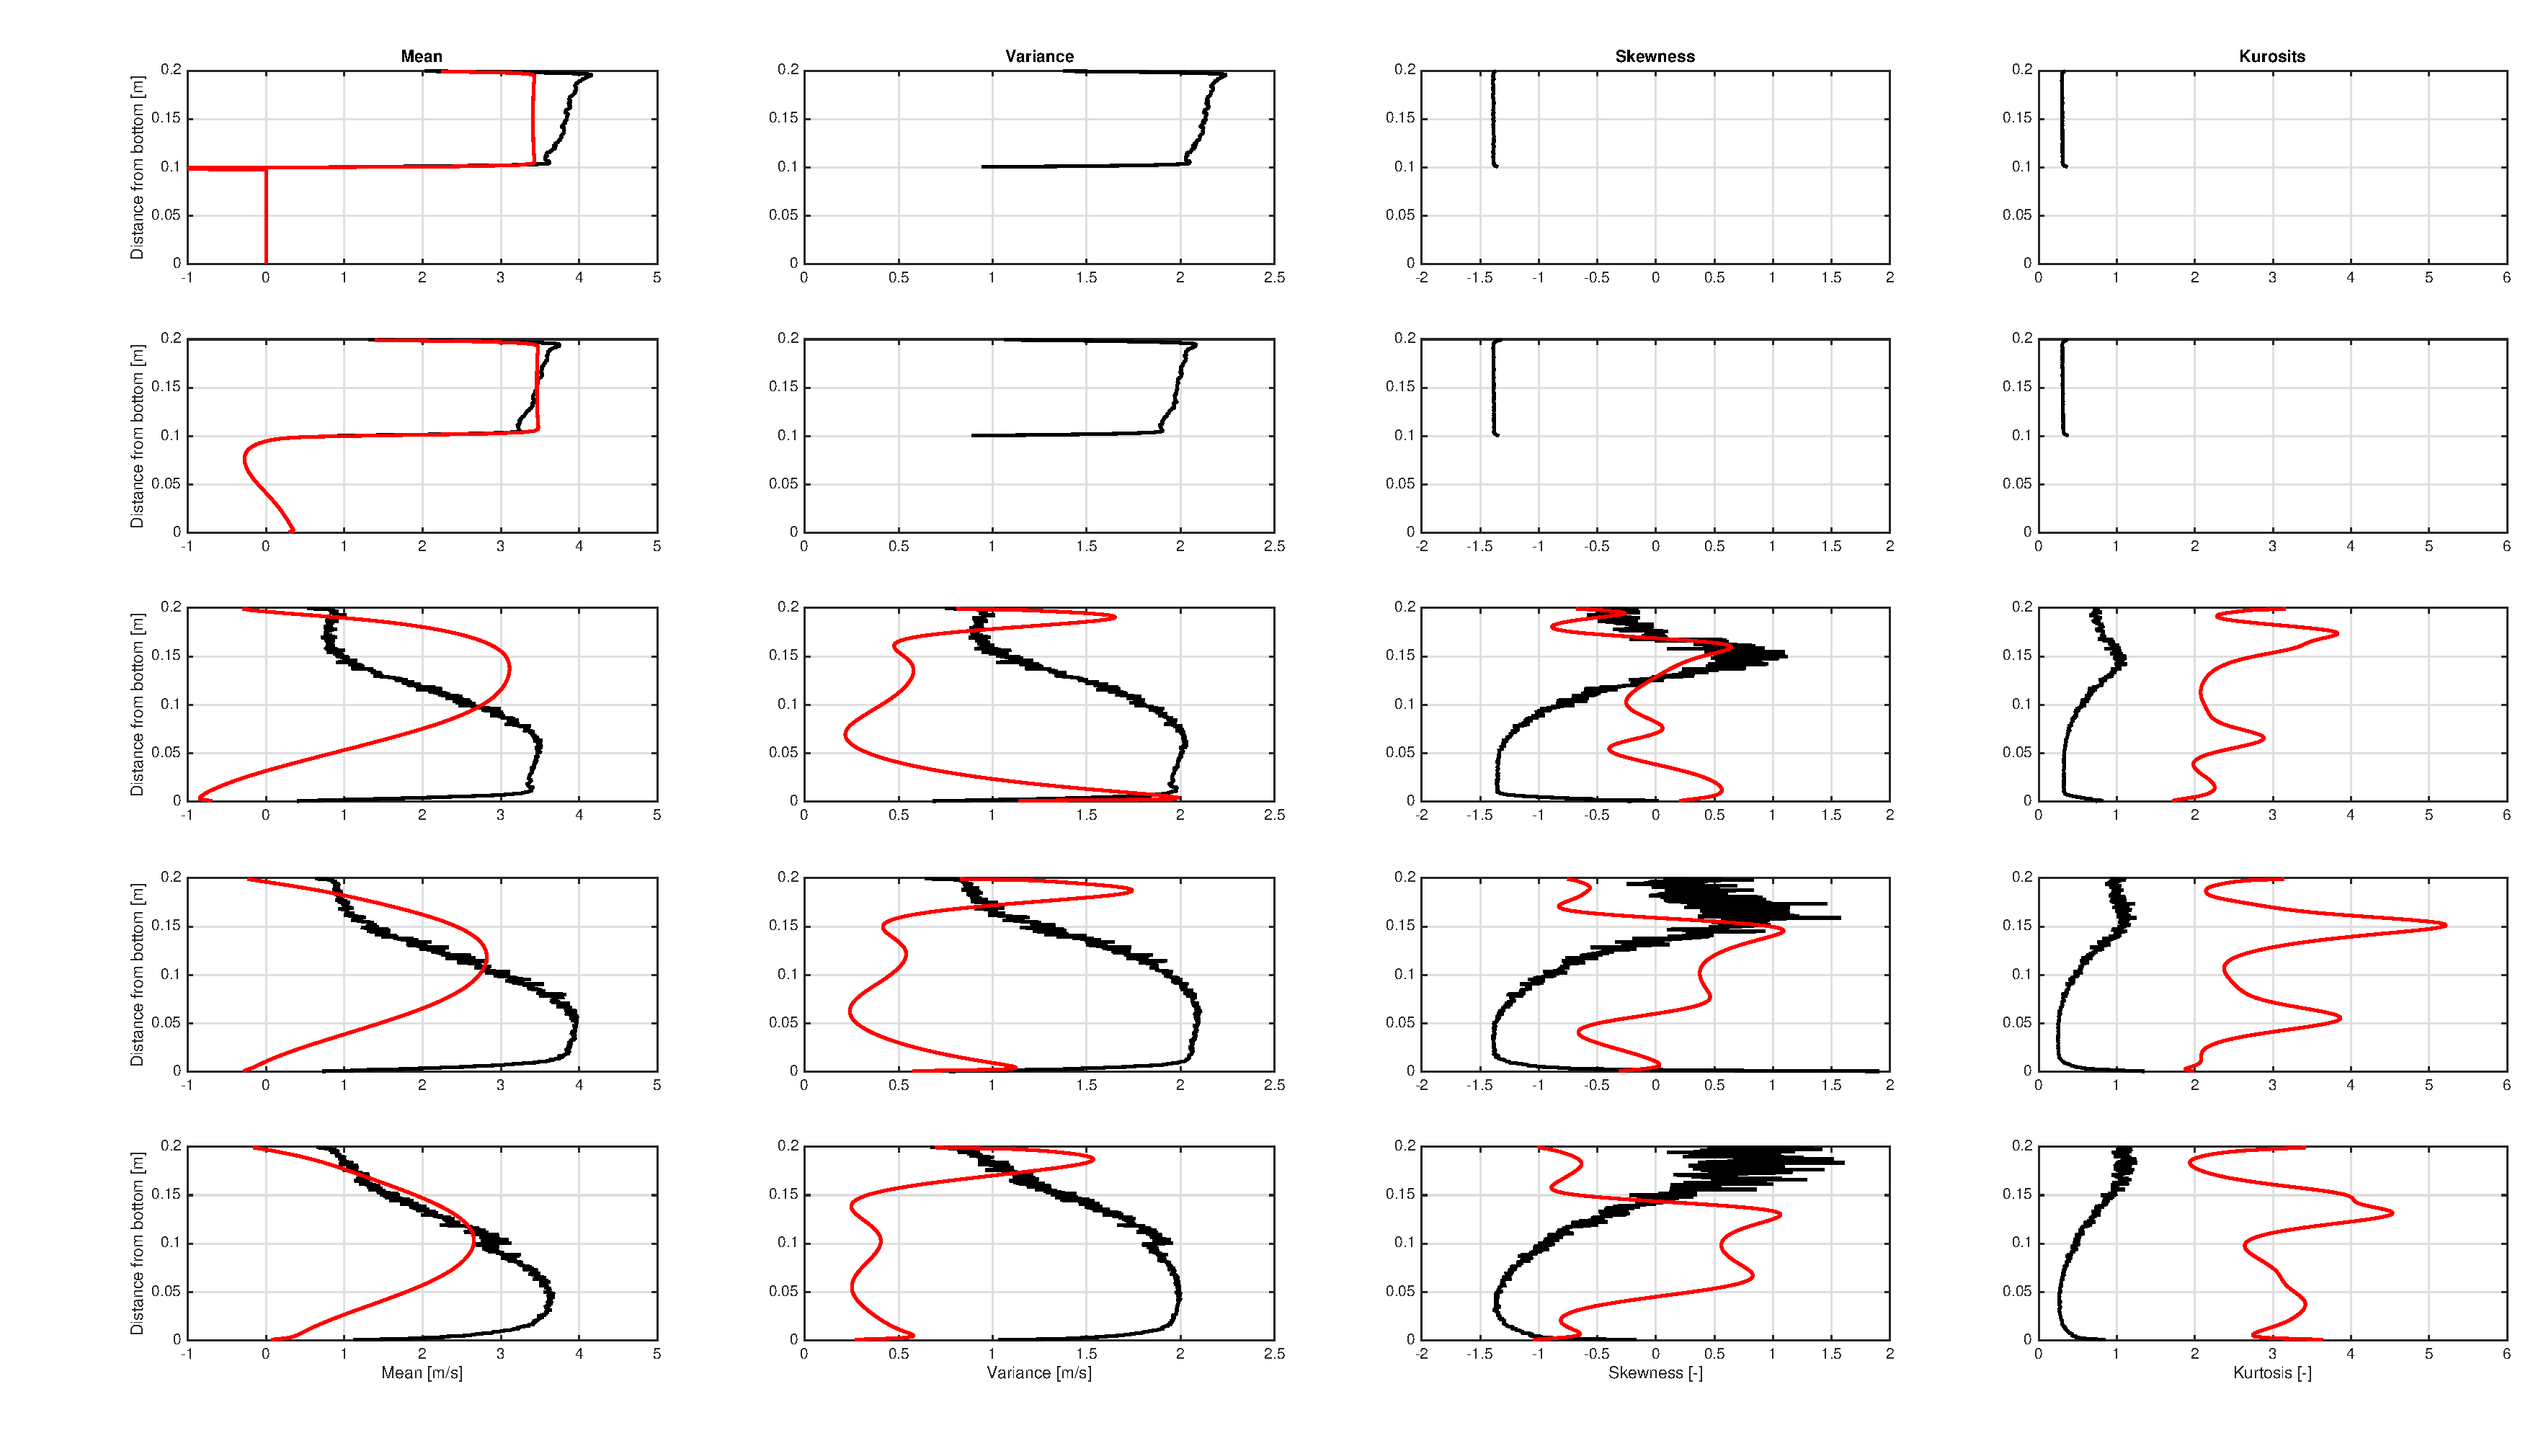
\includegraphics[trim=0 0 0 0,clip,angle=90,width=0.8\textwidth]{FIGURES/Re00_dns.eps}
\caption{Stochastic analysis and comparison for $u=3.372m/s$ for different x-positions}
\label{fig:bfsA}
\end{figure} 

\begin{figure}[!htb]
\centering
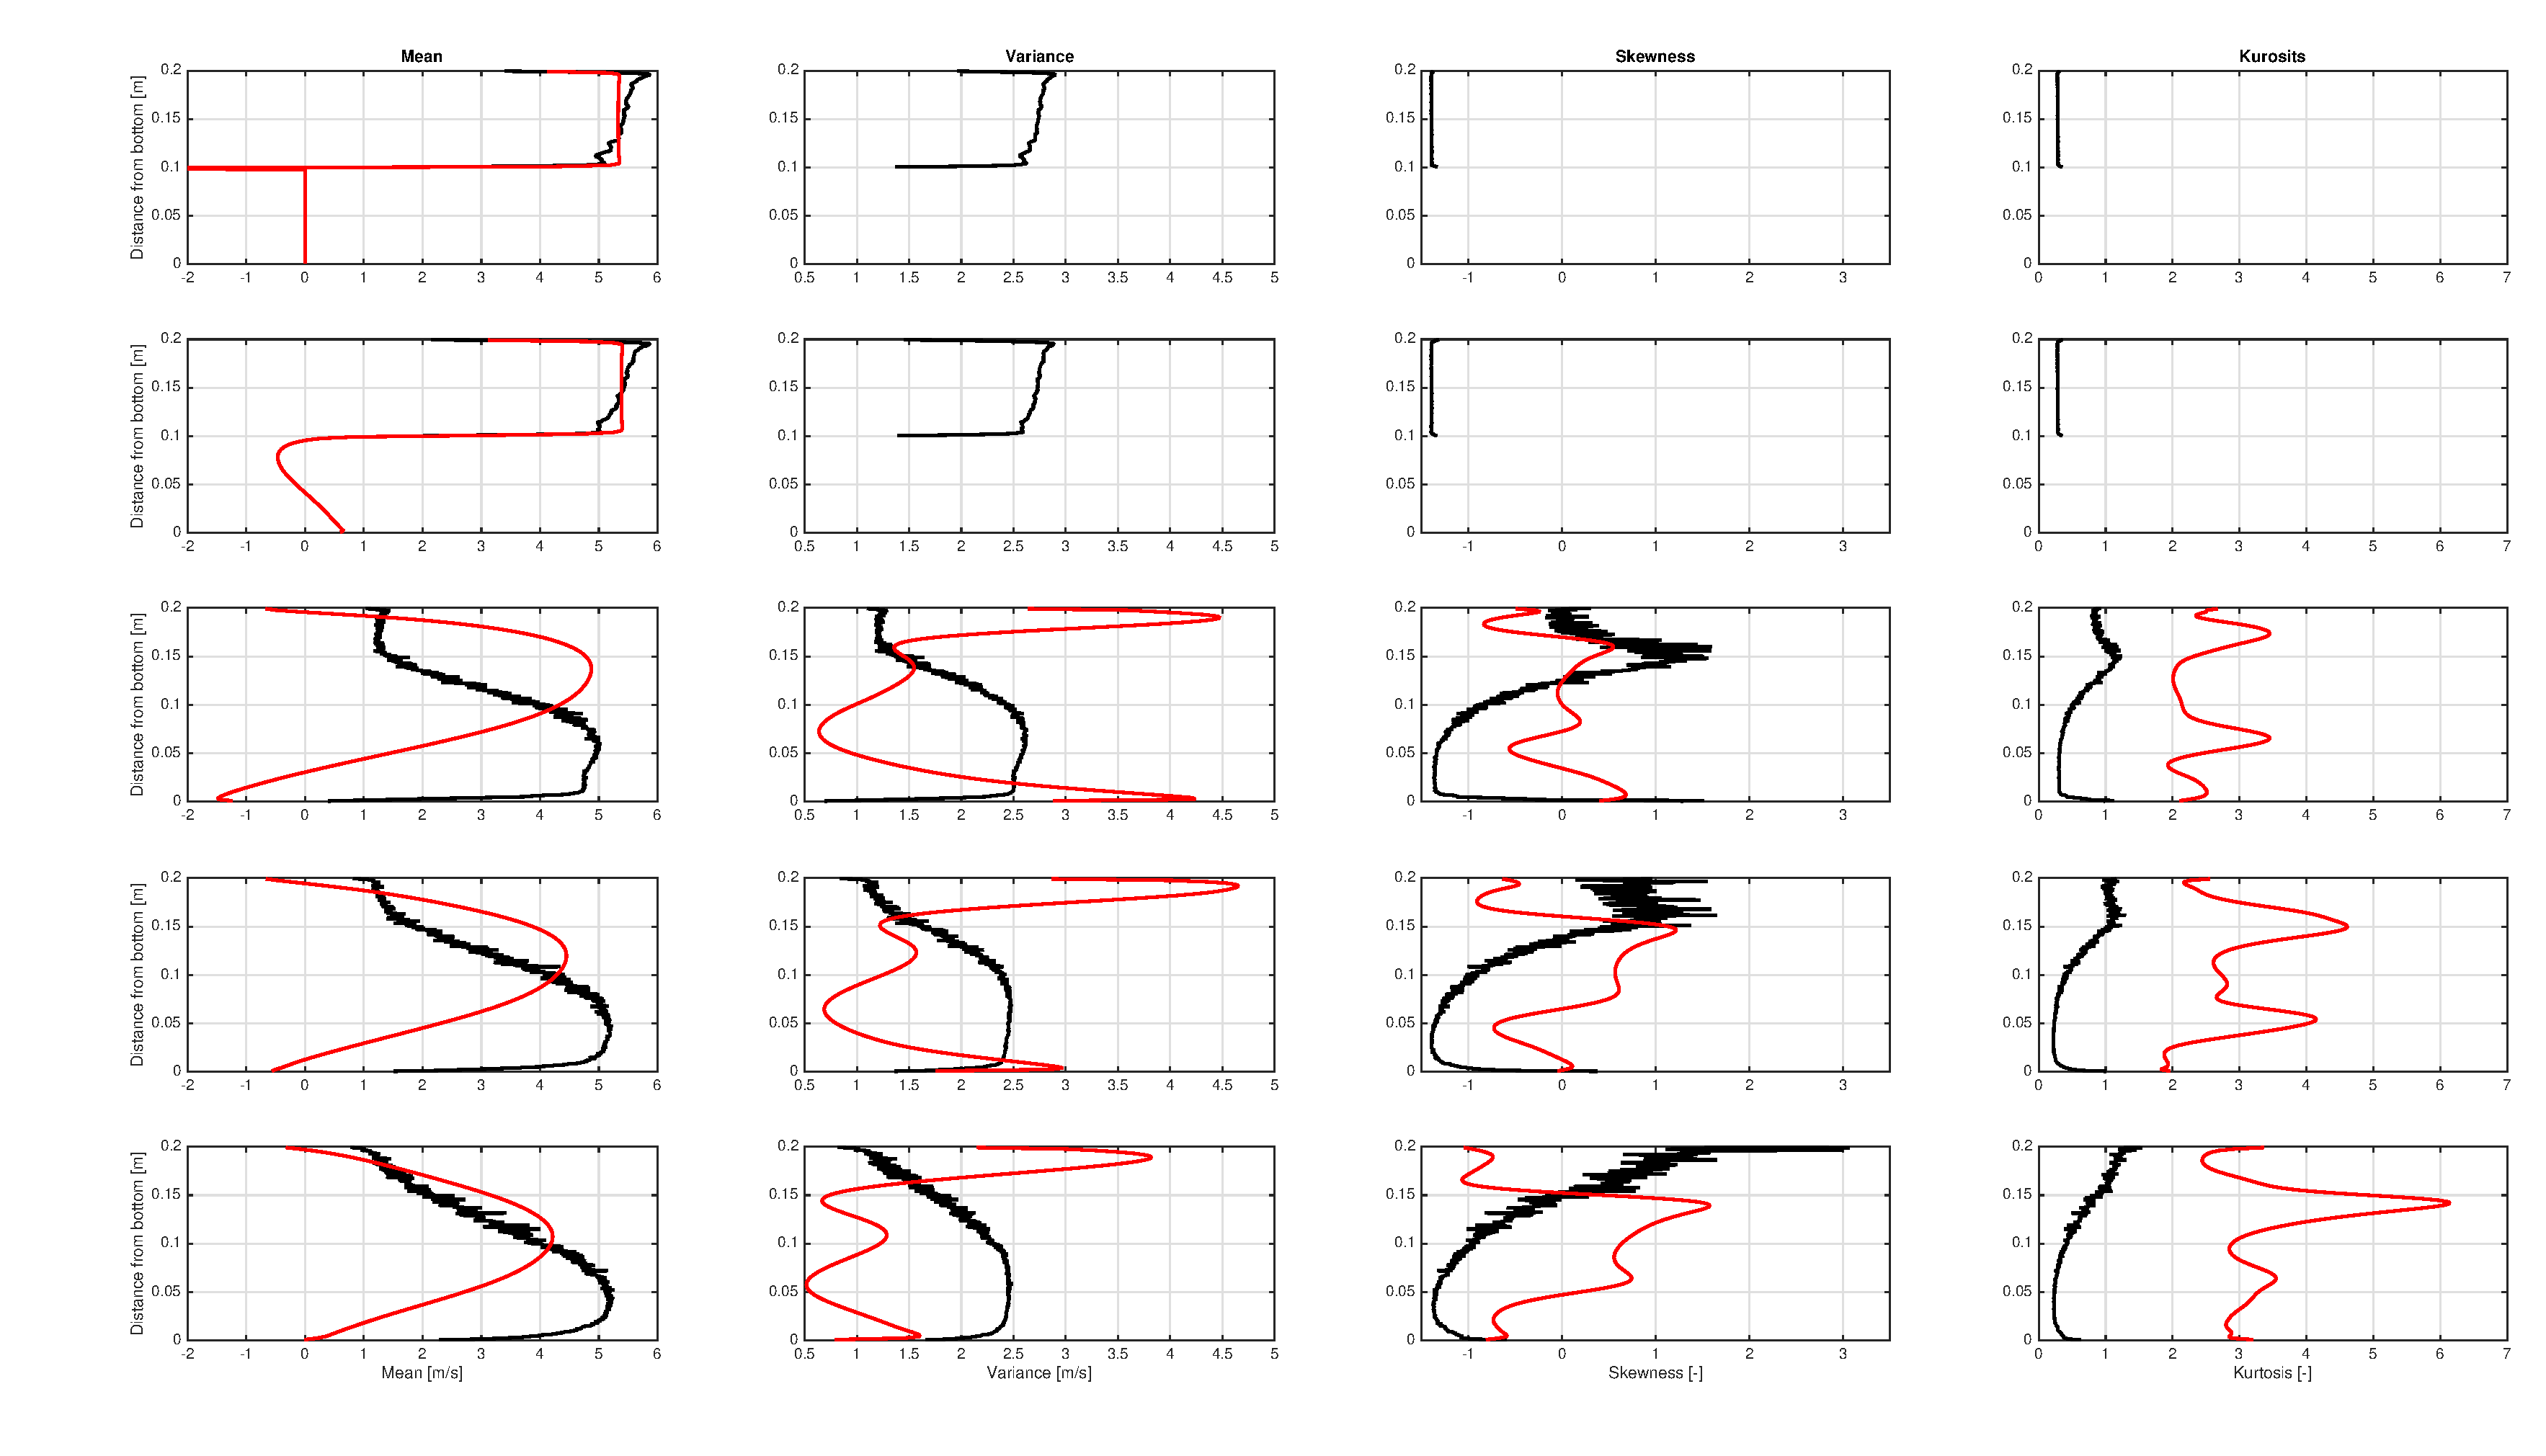
\includegraphics[trim=0 0 0 0,clip,angle=90,width=0.8\textwidth]{FIGURES/Re01_dns.eps}
\caption{Stochastic analysis and comparison for $u=5.295m/s$ for different x-positions}
\label{fig:bfsB}
\end{figure} 

\begin{figure}[!htb]
\centering
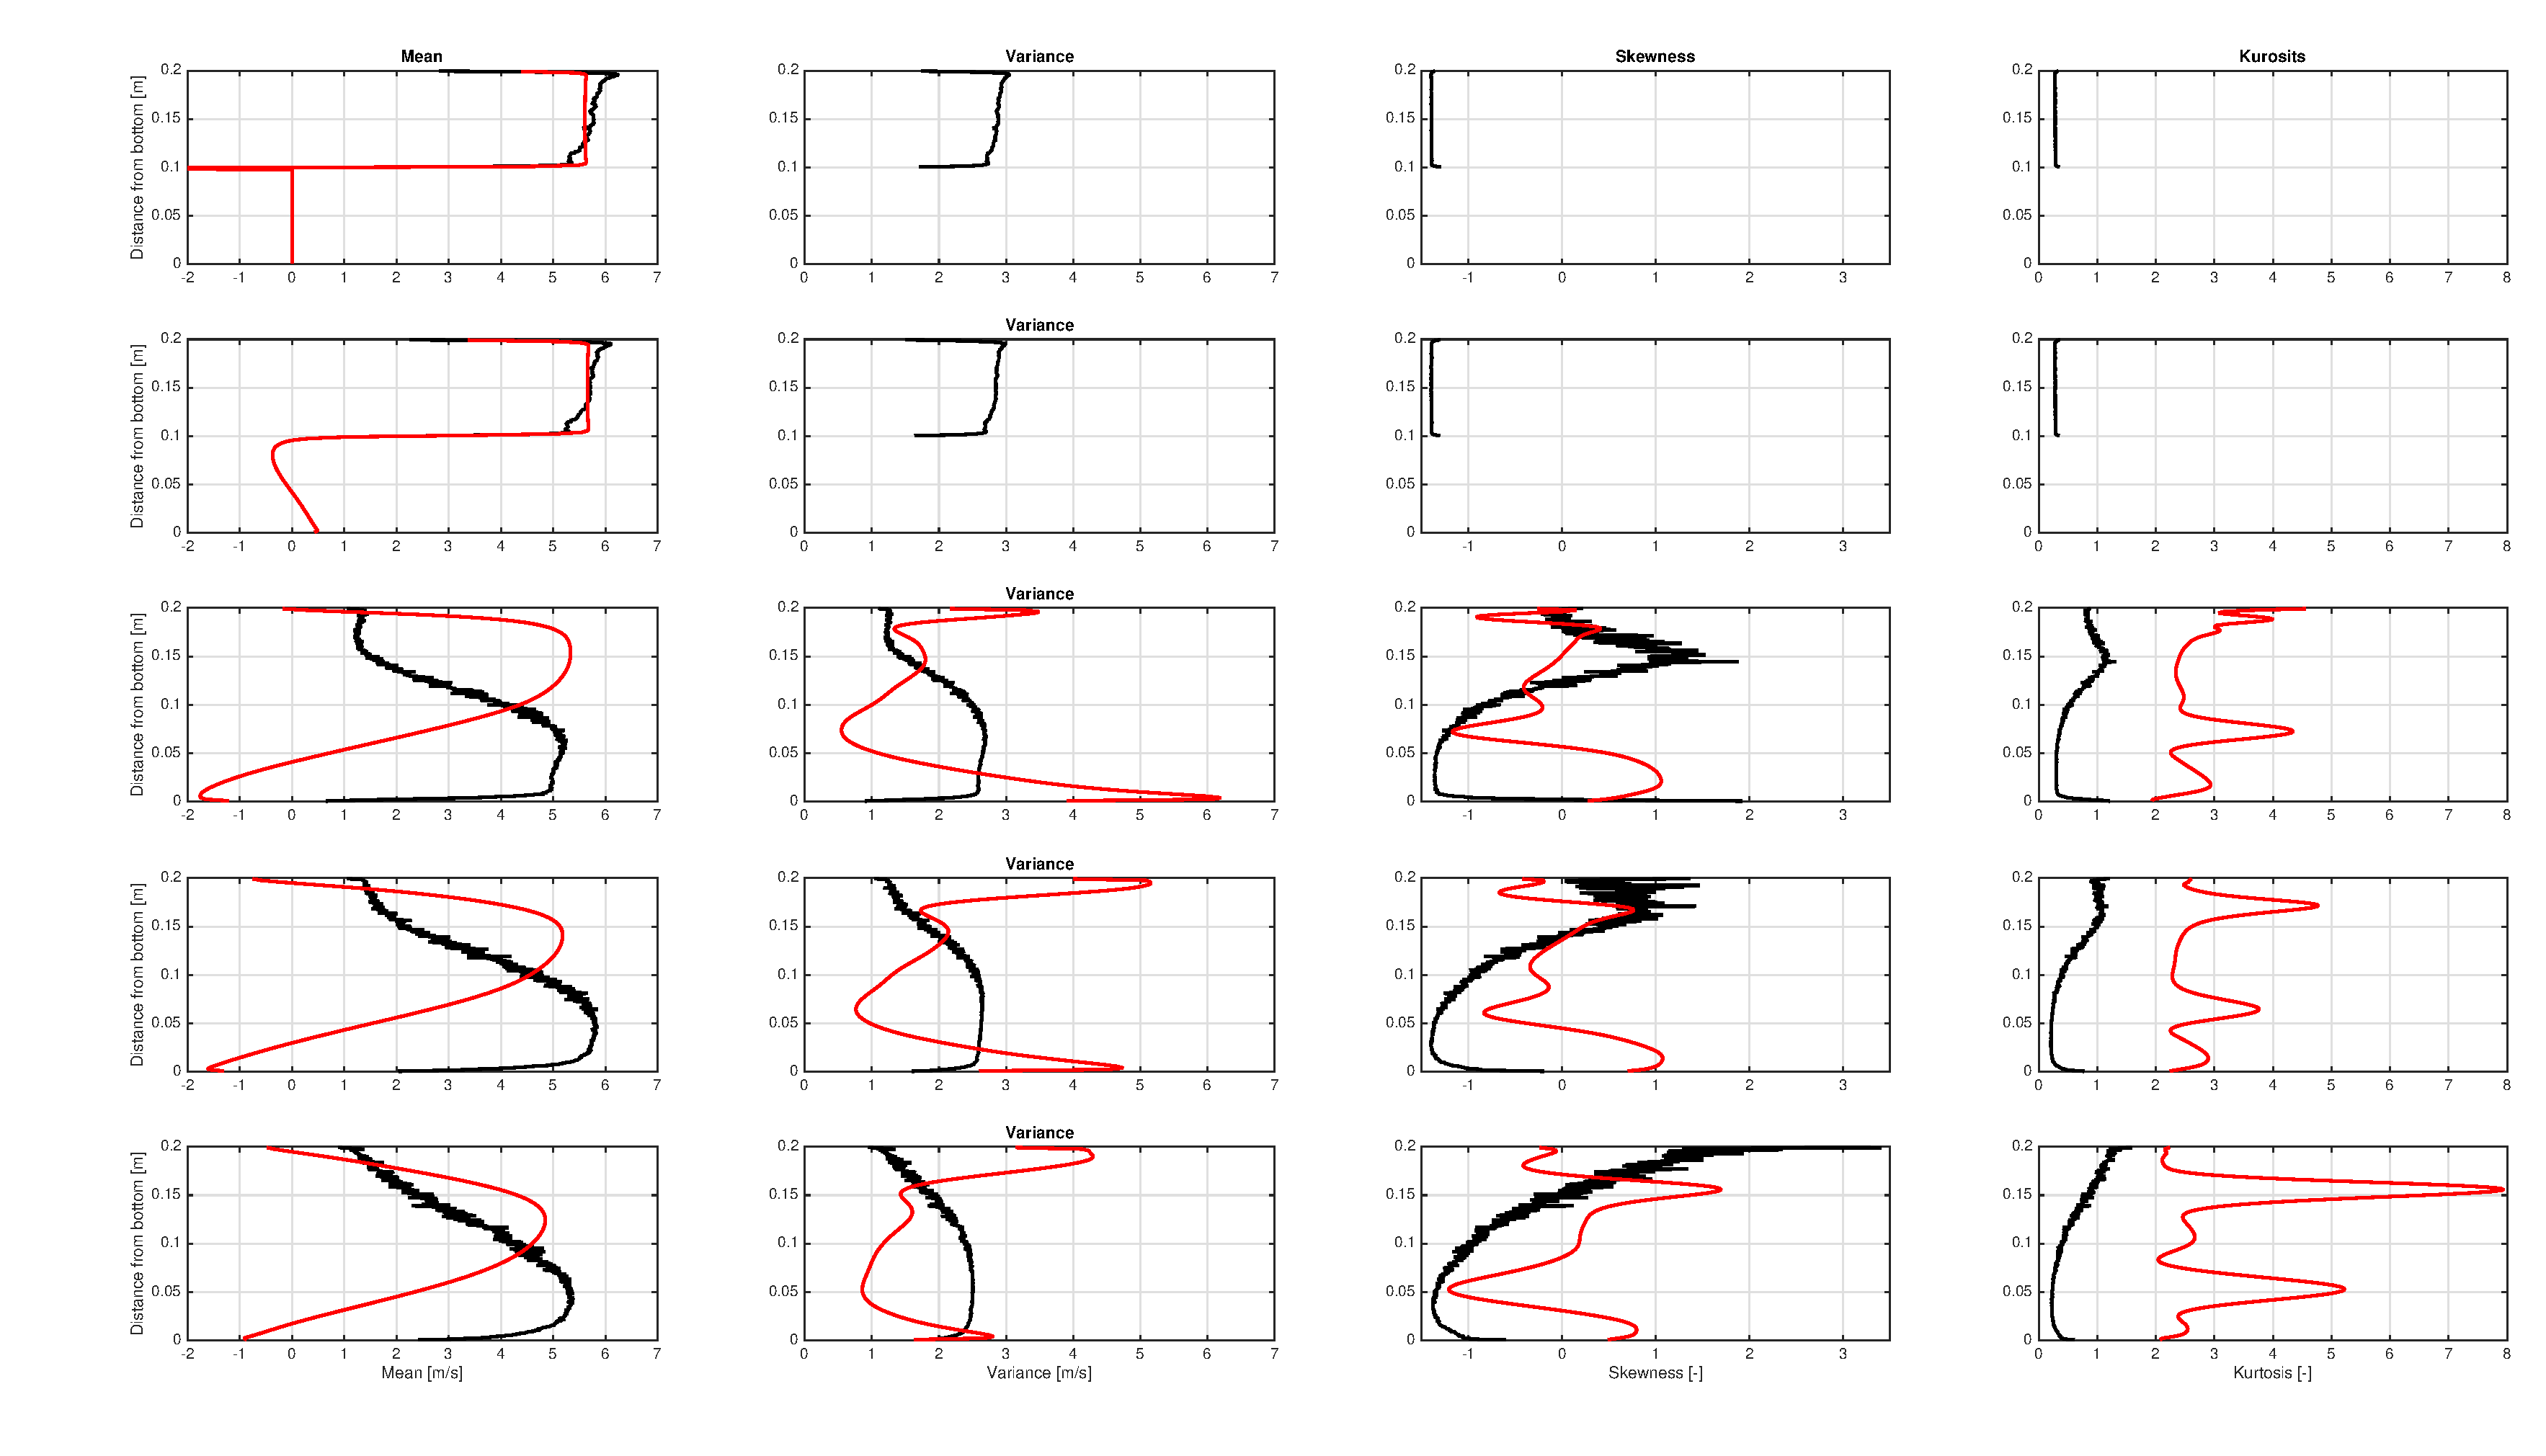
\includegraphics[trim=0 0 0 0,clip,angle=90,width=0.8\textwidth]{FIGURES/Re02_dns.eps}
\caption{Stochastic analysis and comparison for $u=5.579m/s$ for different x-positions}
\label{fig:bfsC}
\end{figure} 

\clearpage
\subsubsection*{Turbulent simulations}

A simulation of the given backward facing step was performed with the algebraic and the \ke\, turbulence model for $u=5.579m/s$. In none of the simulations, instabilities were encountered. No stochastic analysis was needed.

\noii The tendency that the jet prefers the bottom wall could not be encountered in this simulations either (see figure~\ref{fig:bfsprofile}).

\begin{figure}[!htb]
\centering
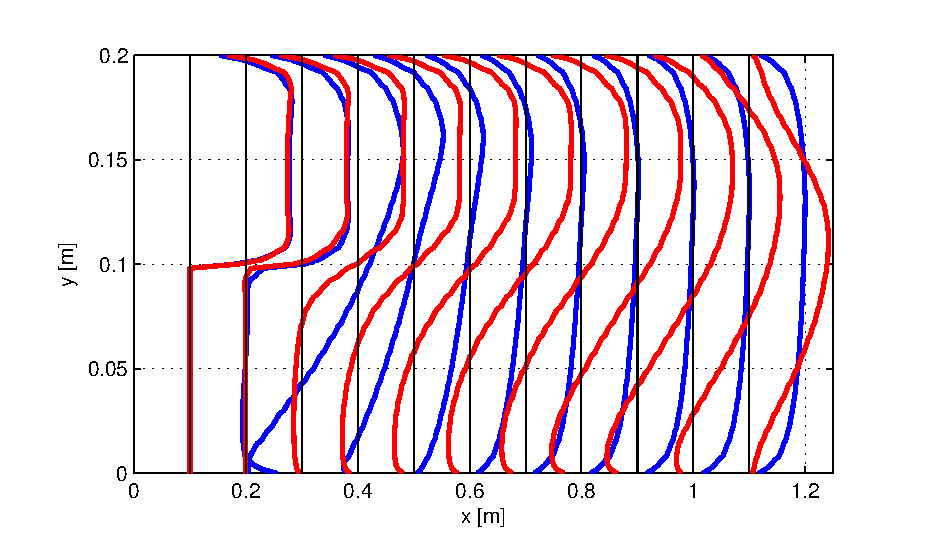
\includegraphics[trim=0 0 0 0,clip,width=0.8\textwidth]{FIGURES/bfs-profile.eps}
\caption{Velocity component in x-direction for (blue) algebraic and (red) \ke-simulation}
\label{fig:bfsprofile}
\end{figure} 



\noii The reattachment occurs in the algebraic simulation between positions C and D and in the \ke\,simulation far behind E. The unsatisfying result of the \ke\,simulation might be due to an underestimated eddy viscosity directly behind the step corner due to a limitation of $\nu_T<\nu\cdot 100$ (see figure~\ref{fig:bfsnut}).

\begin{sidewaysfigure}
%\begin{figure}[!htb]
\centering
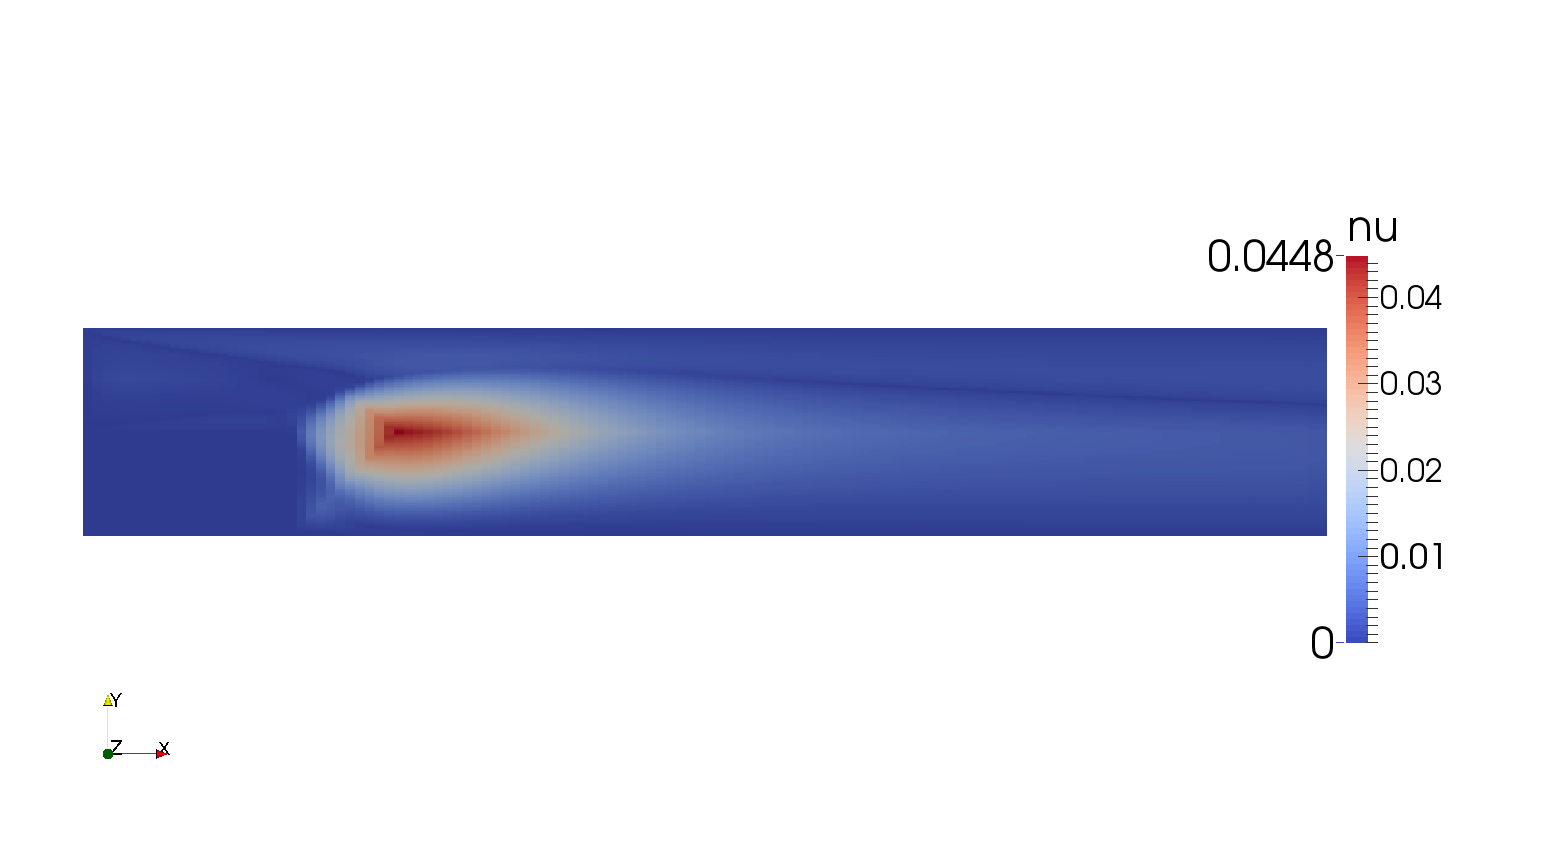
\includegraphics[trim=0 200 0 200,clip,width=1.0\textwidth]{FIGURES/bfs-aturb.png}
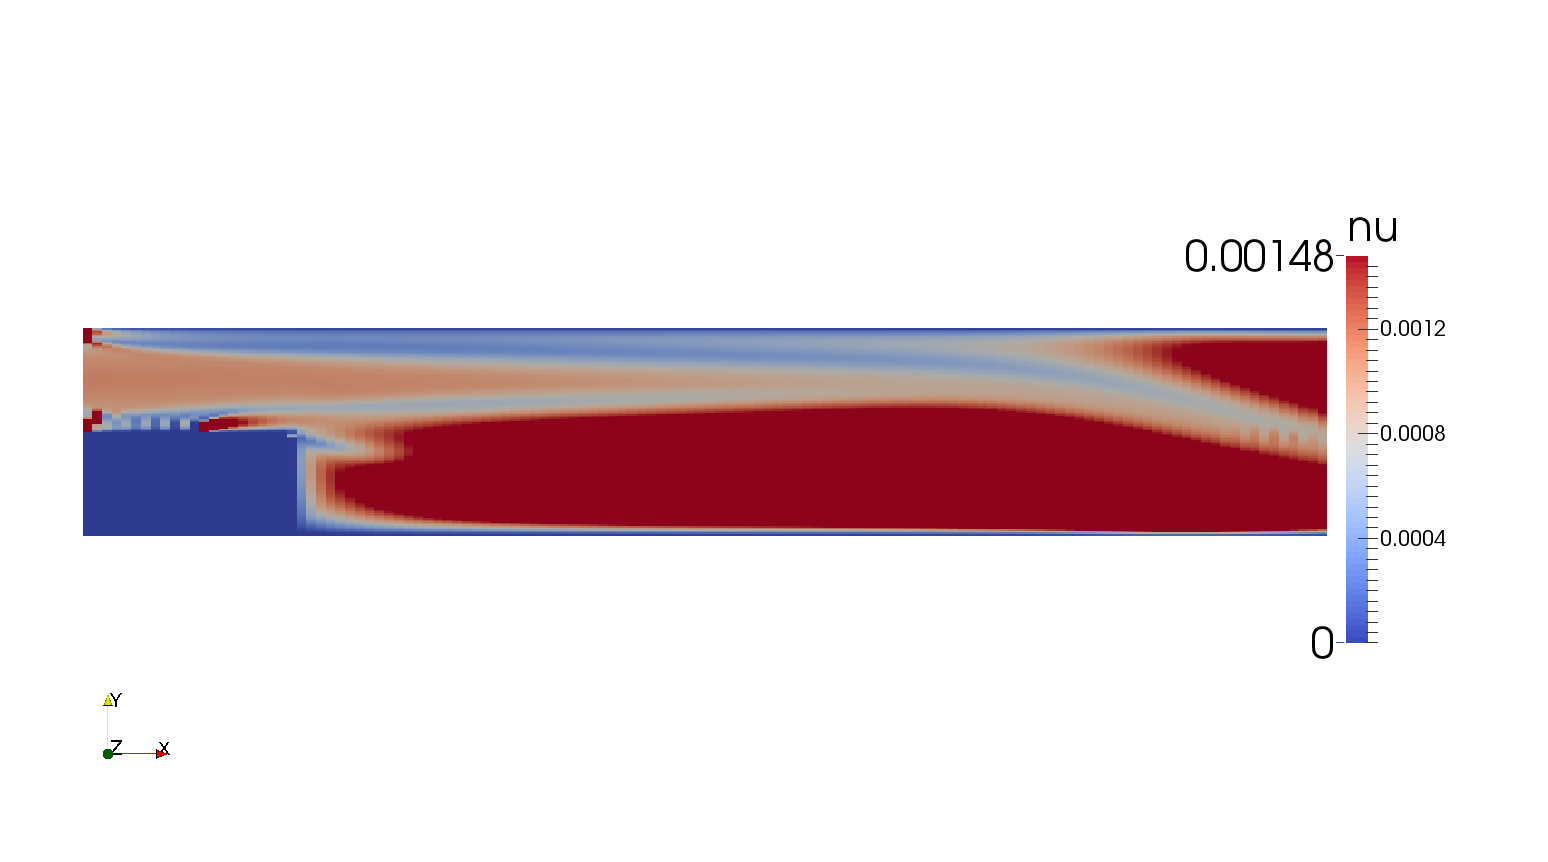
\includegraphics[trim=0 200 0 200,clip,width=1.0\textwidth]{FIGURES/bfs-ke.png}
\caption{Contour plots of the eddy viscosity (top: algebraic, bottom: \ke)}
\label{fig:bfsnut}
%\end{figure} 
\end{sidewaysfigure}

% subsection backward_facing_step (end)

\clearpage
\section{K\'{a}rm\'{a}n vortex street - flow around a cylinder in a channel} % (fold)
\label{sec:karman_vortex_street_flow_around_a_cylinder_in_a_channel}

A cylinder (2D) was used to test how well the import of an arbitrary geometry works. The flow pattern in the wake of the cylinder is a well known and well studied phenomenon (K\'{a}rm\'{a}n vortex street). Measurements from an experiment conducted in a G\"ottingen-type wind tunnel during the lab course 'Praktikum Experimentelle Str\"omungsmechanik' 2015 was used to test the results for validity (see \citep{koehler2015}).

\noii The results of two simulations are presented here. The setup is chosen according to the experimental setup. The two simulations differ only in the chosen scenario: 1) channel and 2) free. It was seen that the chosen boundary conditions have clear influence on the flow patterns\footnote{It was not possible to simulate a big enough flow field, so that no influence of the boundary conditions could be noticed: the code needs to be extended for parallel simulations to be able to handle an appropriate mesh size.}.




\begin{center}
\begin{tabular}{lccc}
\hline 
Re                   & 61814\\      
Uniform velocity profile $u$         & 10 \\
Geometry (Flow field)  &  1$\times$0.2\\
Geometry (Cylinder)  &  x=0.2, y=0.1, d=0.03\\
Mesh Type & uniform \\
Mesh      & 256\,$\times$\,256 \\\hline 
\end{tabular}
\end{center}

\noii The 'animation' figure~\ref{fig:karman-ani1} shows how the flow develops from the initial condition (no flow) to the periodic flow condition with well visible vortex street  and \ref{fig:karman-ani2} shows a fully developed vortex street. The vortex shedding frequency matches well with the expected value:
\begin{align*}
f=\frac{Sr \cdot u}{d}=66.7Hz \qquad \text{with } Sr\approx0.2
\end{align*}

\noii Figure~\ref{fig:karman-stoch2} shows the stochastic analysis along a path downstream of cylinder with a distance $\Delta x = 0.100$. The stochastic analysis of the measured values are plotted in figure~\ref{fig:karman-stoch1}. The overall tendencies of the modes are both in the simulation and in the measurements similar. The influence of the boundary conditions is clearly visible leading to the discrepancies. For detailed evaluation of the experimental results (among other things modes along a path behind a cylinder), we would like to refer interested readers to \citep{koehler2015}. 

\newcommand{\inkarman}[1]{\includegraphics[trim=0 250 0 250,clip,width=0.8\textwidth]{#1}}

\begin{figure}[!htb]
\centering
\inkarman{FIGURES/karman10.png}
\inkarman{FIGURES/karman20.png}
\inkarman{FIGURES/karman30.png}
\inkarman{FIGURES/karman40.png}
\inkarman{FIGURES/karman50.png}
\inkarman{FIGURES/karman60.png}
\inkarman{FIGURES/karman70.png}
\caption{First 70ms with a sample rate of 100Hz}
\label{fig:karman-ani1}
\end{figure} 

\begin{figure}[!htb]
\centering
\inkarman{FIGURES/k1000.png}
\inkarman{FIGURES/k1001.png}
\inkarman{FIGURES/k1002.png}
\inkarman{FIGURES/k1003.png}
\inkarman{FIGURES/k1004.png}
\inkarman{FIGURES/k1005.png}
\inkarman{FIGURES/k1006.png}
\caption{Fully developed vortex street: part of a full periode (sample rate 100Hz)}
\label{fig:karman-ani2}
\end{figure} 

\begin{figure}[!htb]
\centering
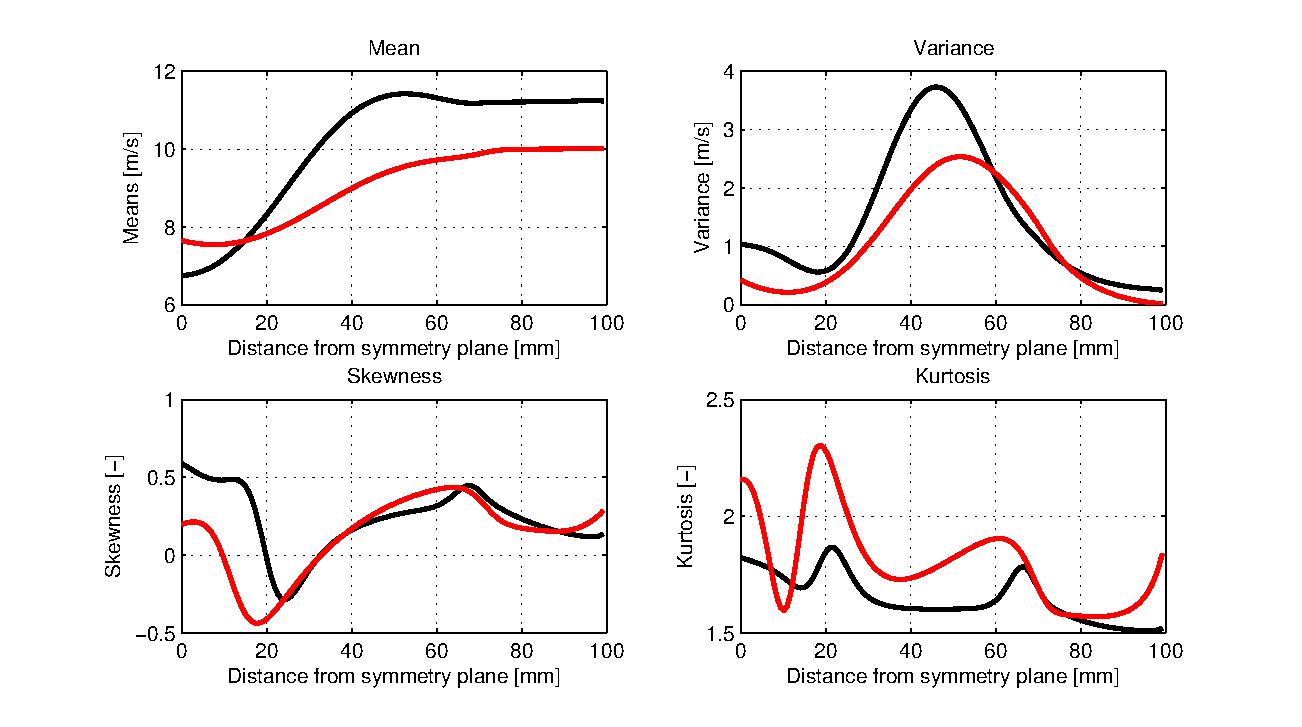
\includegraphics[trim=10 0 10 0,clip,width=1.0\textwidth]{FIGURES/karman-stoch.eps}
\caption{Stochastic analysis of the simulation results along a path 100mm behind the cylinder (black: channel, red: free)}
\label{fig:karman-stoch2}
\end{figure} 


\begin{figure}[!htb]
\centering
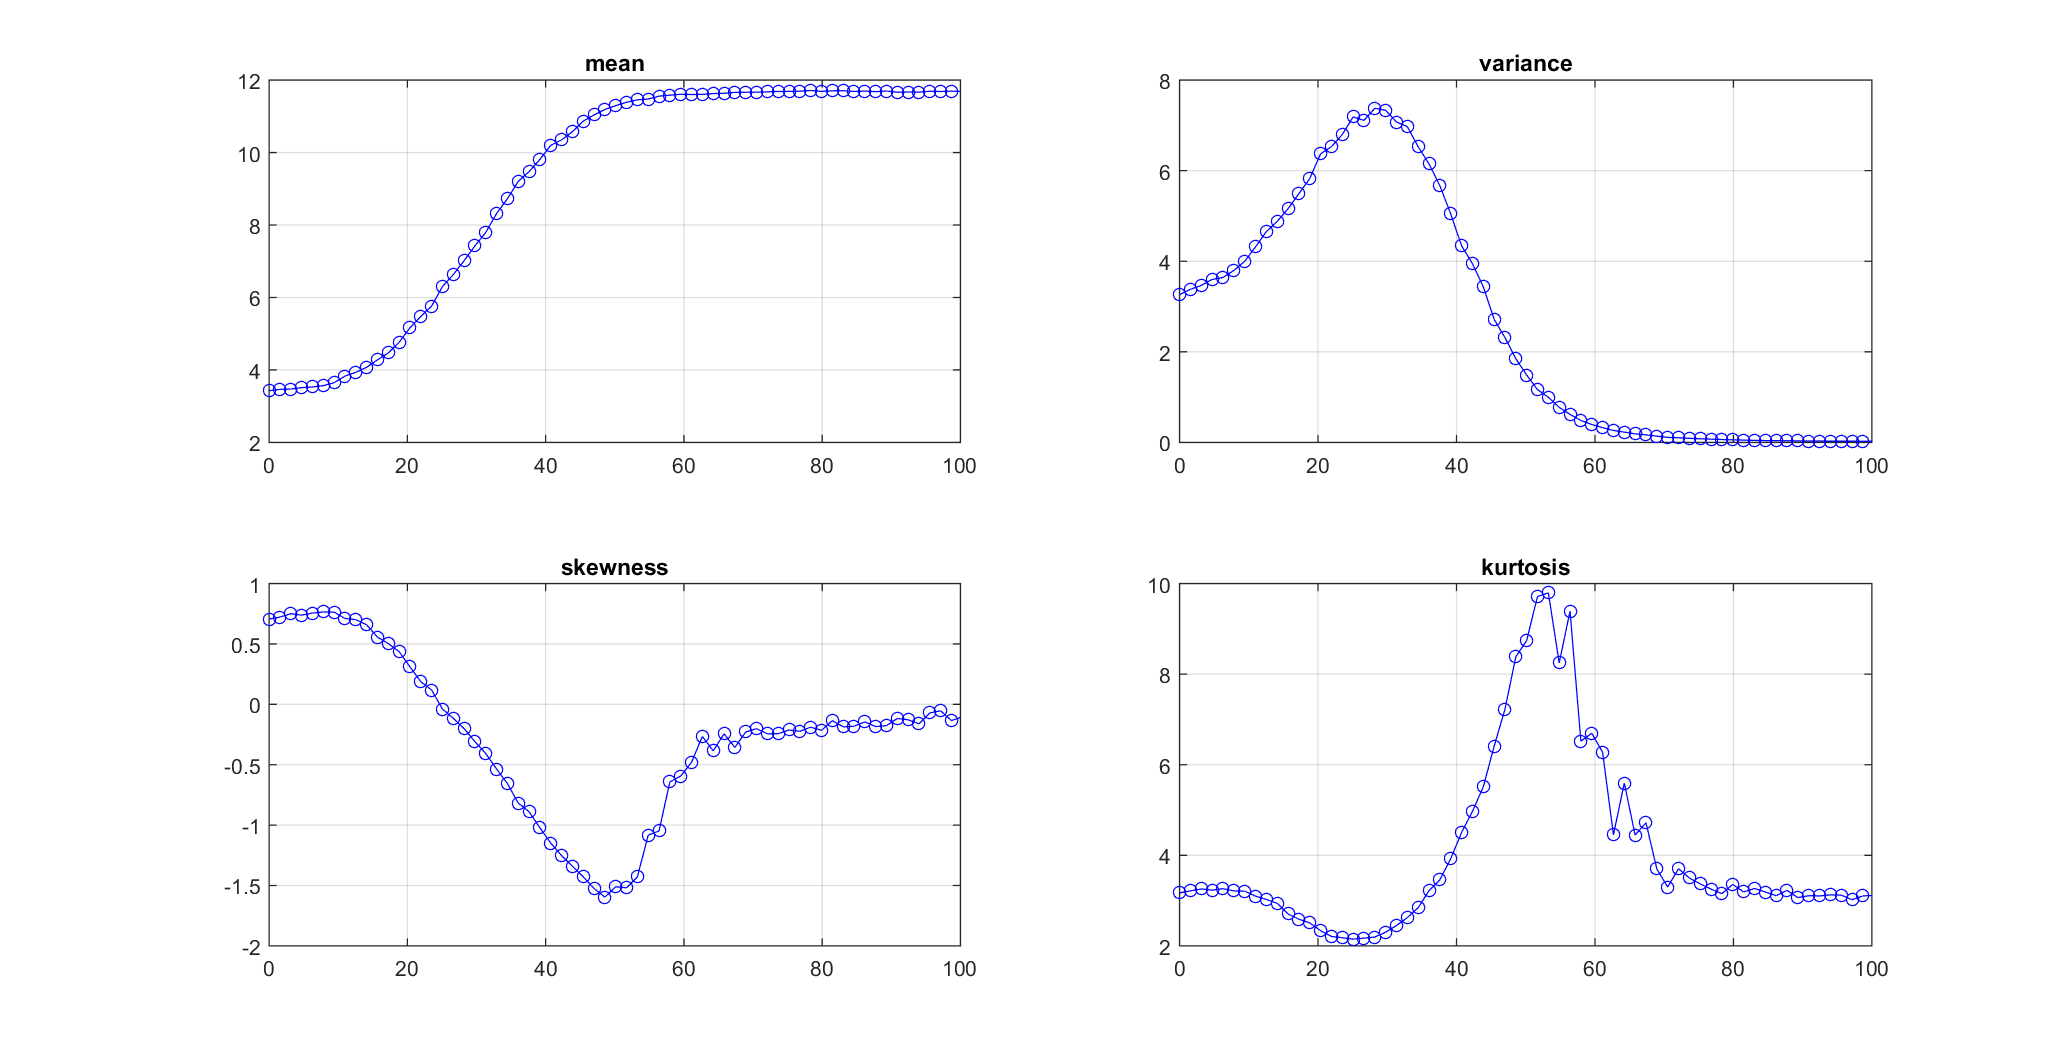
\includegraphics[trim=80 0 80 0,clip,width=1.0\textwidth]{FIGURES/wake-ana.png}
\caption{Stochastic analysis of the experimental measurement along a path 100mm behind the cylinder}
\label{fig:karman-stoch1}
\end{figure} 





% subsection karman_vortex_street_flow_around_a_cylinder_in_a_channel (end)

% chapter numerical_results (end)